\section{Geometria Plana}


\subsection*{Equações Cartesianas da reta em $\R^2$}

%%%%%%%%%%%%%%%%%%%%%%%%%%%%%%%%%%%%%%%%%%%%%%%%%%%%%%%%%%%%
\begin{frame}[label=retas]{O conjunto $\R^2$}

O {\color{blue} \(\R^2\)}  é o conjunto   formado pelos {\color{blue}pares ordenados} $(x,y)$ tais $x$ e $y$ são números reais, isto é,
\[{\color{blue} \R^2}=\{(x,y);\ x,y\in \R\} \]

 O número $x$ chama-se {\color{blue}primeira coordenada ou abcissa} e o número $y$ chama-se {\color{blue}segunda coordenada ou ordenada}. 
\medskip


\end{frame}
%%%%%%%%%%%%%%%%%%%%%%%%%%%%%%%%%%%%%%%%%%%%%%%%%%%%%%%%%%%%
\begin{frame}[label=retas]{Interpretação Geométrica do conjunto $\R^2$}
Podemos representar geometricamente os elementos de {\color{blue} \(\R^2\)}  usando um {\color{blue}sistema de coordenadas cartesianas}, que consiste em um plano com um par de eixos perpendiculares $OX$ e $OY$ e que tem a mesma origem.

		\begin{figure}[h]
	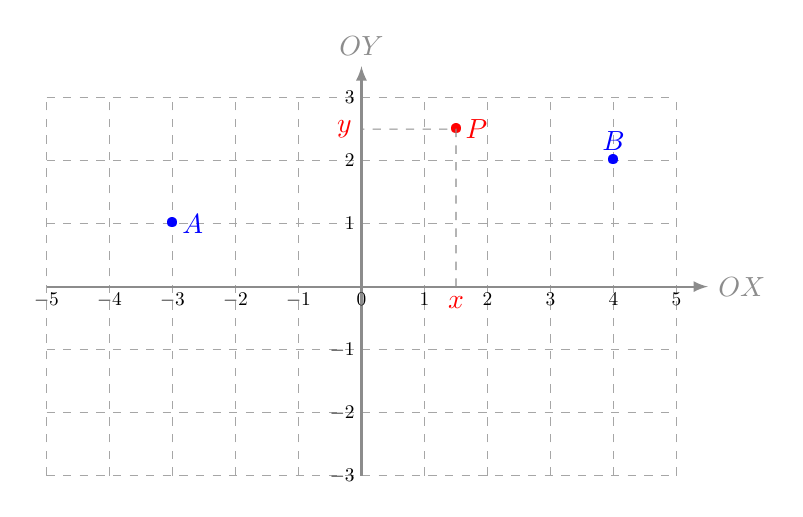
\begin{tikzpicture}[scale=0.8]
	\tikzset{>=latex}
	\draw[help lines, color=gray!70, dashed] (-5,-3) grid (5,3);
	\draw[->,thick,color=gray!90] (-5,0)--(5.5,0) node[right]{$OX$};
	\draw[->,thick,color=gray!90] (0,-3)--(0,3.5) node[above]{$OY$};
	\foreach \i in {-5,...,5}
	\node[below,scale=0.7] at (\i,0) {$\i$};
	\foreach \i in {-3,...,-1}
	\node[left,scale=0.7] at (0,\i) {$\i$};
	\foreach \i in {1,...,3}
	\node[left,scale=0.7] at (0,\i) {$\i$};
	
	\coordinate (X) at (1.5,2.5);
	\coordinate (A) at (-3,1);
	\coordinate (B) at (4,2);

	\node[red] at (X) {\textbullet};
	\draw[color=gray!90,dashed] (1.5,0)--(X)--(0,2.5) ;
	\node[red,right] at (X) {$P$};
	\node[red,below] at (1.5,0) {$x$};
	\node[red,left] at (0,2.5) {$y$};

	\node[blue] at (A) {\textbullet};
	\node[blue,right] at (A) {$A$};
	
	\node[blue] at (B) {\textbullet};
	\node[blue,above] at (B) {$B$};
	
	
	%	\node[blue] at (Q) {\textbullet};
	%	\node[blue,above] at (Q) {$Q$};
	
	\end{tikzpicture}
\end{figure}

\end{frame}
%%%%%%%%%%%%%%%%%%%%%%%%%%%%%%%%%%%%%%%%%%%%%%%%%%%%%%%%%%%%

\begin{frame}[label=retas]


\begin{exe}
Em um plano, fixado um sistema de coordenadas cartesianas, represente:
\begin{enumerate}
\item Os pontos $P=(1,0)$, $Q=(2,1)$ e $R=(-3,-2)$.
\item Os conjuntos $A=\{(x,y)\in \R^2;\ x=1\}$ e $B=\{(x,y)\in \R^2;\ x=y\}$.
\end{enumerate}
\end{exe}
\end{frame}
%%%%%%%%%%%%%%%%%%%%%%%%%%%%%%%%%%%%%%%%%%%%%%%%%%%%%%%%%%%
\begin{frame}[label=retas]{Equações da Reta no \(\R^2\)}

As coordenadas de um ponto qualquer {\color{blue}\(P=(x,y)\)} da reta que passa pelo ponto {\color{blue} \( A=(x_0,y_0)\)} e faz um ângulo  {\color{red}\(\alpha\) } com o eixo dos \(x\) satisfazem a seguinte equação:
\[
{\color{blue}y-y_0}={\color{red}m}{\color{blue}(x-x_0)},
\]
onde {\color{red}\(m=\tan(\alpha)\)}.

		\begin{figure}[h]
	\begin{tikzpicture}[scale=0.7]
	\tikzset{>=latex}
	\draw[help lines, color=gray!70, dashed] (-5,-3) grid (5,3);
	\draw[->,thick,color=gray!90] (-5,0)--(5.5,0) node[right]{$OX$};
	\draw[->,thick,color=gray!90] (0,-3)--(0,3.5) node[above]{$OY$};

	\pgfmathsetmacro{\xo}{1}
    \pgfmathsetmacro{\yo}{1}
	\pgfmathsetmacro{\x}{3}
    \pgfmathsetmacro{\y}{2}
	\coordinate (A) at (\xo,\yo);
	\coordinate (X) at (\x,\y);
	\coordinate (B) at (\x,\yo);
%$(A)!fator!(X)$ encontre um ponto na linha entre A e X, onde o fator determina a posição relativa
\draw[blue,thick] ($(A)!-3!(X)$) -- ($(A)!2!(X)$);

	\node[blue] at (A) {\textbullet};
	\node[blue,above] at (A) {\(A\)};
	\node[blue,below] at (\xo,0) {$x_0$};
	\node[blue,left] at (0,\yo) {$y_0$};

	
    \node[blue] at (X) {\textbullet};
	\node[blue,below] at (\x,0) {$x$};
	\node[blue,left] at (0,\y) {$y$};

	\node[red] at (2.5,1.3) {$\alpha$};
	\pic[draw, angle radius=8mm, angle eccentricity=1.2, red, thick] {angle = B--A--X};

	\end{tikzpicture}
\end{figure}


\end{frame}


%%%%%%%%%%%%%%%%%%%%%%%%%%%%%%%%%%%%%%%%%%%%%%%%%%%%%%%%%%%%	
\begin{frame}[label=retas]{Equações reduzida da Reta no \(\R^2\)}
	\begin{block}{Equação reduzida da reta}
		A equação de uma reta é chamada de   \dest{equação reduzida} quando  está na seguinte forma:
		\[y={\color{red}m}x+n.\]
		O coeficiente  {\color{blue}\(m\)} é dito {\color{red}coeficiente angular} da reta e mede a tangente do ângulo que a reta faz com o eixo $OX$. E o número $n$ é dito \dest{coeficiente linear} da reta e representa a ordenada do ponto de interseção da reta com o eixo $OY$.
	\end{block}

	\begin{exe}\noindent
  Encontre a equação cartesiana da reta que passa pelos pontos $P=(1,3)$ e $Q=(5,-9)$.
	\end{exe}

\end{frame}
%%%%%%%%%%%%%%%%%%%%%%%%%%%%%%%%%%%%%%%%%%%%%%%%%%%%%%%%%%%%

\begin{frame}
	
	%\begin{scriptsize}
	\begin{block}{Equação segmentária da reta}
		A equação de uma reta é chamada de   \dest{equação segmentária}  quando  está na seguinte forma:
		\[\frac{x}{{\color{blue}p}}+\frac{y}{{\color{blue}q}}=1.\]
		Neste caso, a reta intercepta os eixos $OX$ e $OY$ nas coordenadas {\color{blue}$p$} e {\color{blue}$q$} respectivamente. 
	\end{block}
	
	%\end{scriptsize}
\end{frame}

\begin{frame}
	\begin{exe}
	\begin{enumerate}
		\item 	 Determine a equação cartesiana da reta $r$ que passa pelos pontos $A=(0,3)$ e $B=(2,0)$.
		
		
		\item Determine a equação cartesiana da reta que passa pelos pontos $A=(0,1)$ e $B=(2,2)$.
		
		
	\end{enumerate}
	\end{exe}


	\begin{minipage}{0.45\textwidth}
		\begin{figure}[h]
		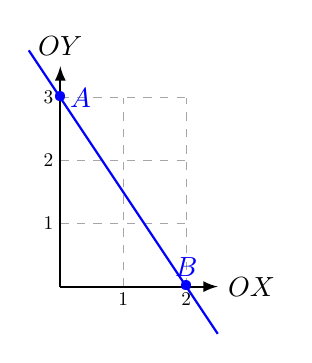
\begin{tikzpicture}[scale=0.8]
	\tikzset{>=latex}
	\draw[help lines, color=gray!70, dashed] (0,0) grid (2,3);
	\draw[->,thick] (0,0)--(2.5,0) node[right]{$OX$};
	\draw[->,thick] (0,0)--(0,3.5) node[above]{$OY$};
	\foreach \i in {1,...,2}
	\node[below,scale=0.7] at (\i,0) {$\i$};
	\foreach \i in {1,...,3}
	\node[left,scale=0.7] at (0,\i) {$\i$};
	
	
	\coordinate (O) at (0,0);
	\coordinate (A) at (0,3);
	\coordinate (B) at (2,0);
	
	
	\node[blue] at (A) {\textbullet};
	\node[blue,right] at (A) {$A$};
	
	\node[blue] at (B) {\textbullet};
	\node[blue,above] at (B) {$B$};
	
	\draw[blue,thick] (-.5,3.75) -- (2.5,-0.75) ;
	
	
	
	%	\node[blue] at (Q) {\textbullet};
	%	\node[blue,above] at (Q) {$Q$};
	
	\end{tikzpicture}
	\caption{Exemplo 1}
	\end{figure}
	\end{minipage}
	\begin{minipage}{0.45\textwidth}
		\begin{figure}[h]
	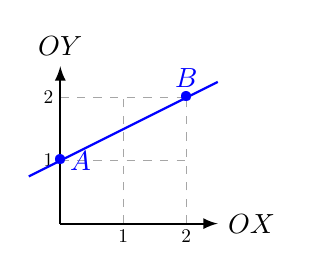
\begin{tikzpicture}[scale=0.8]
	\tikzset{>=latex}
	\draw[help lines, color=gray!70, dashed] (0,0) grid (2,2);
	\draw[->,thick] (0,0)--(2.5,0) node[right]{$OX$};
	\draw[->,thick] (0,0)--(0,2.5) node[above]{$OY$};
	\foreach \i in {1,...,2}
	\node[below,scale=0.7] at (\i,0) {$\i$};
	\foreach \i in {1,...,2}
	\node[left,scale=0.7] at (0,\i) {$\i$};
	
	
	\coordinate (O) at (0,0);
	\coordinate (A) at (0,1);
	\coordinate (B) at (2,2);
	
	
	\node[blue] at (A) {\textbullet};
	\node[blue,right] at (A) {$A$};
	
	\node[blue] at (B) {\textbullet};
	\node[blue,above] at (B) {$B$};
	
	\draw[blue,thick] (-.5,0.75) -- (2.5,2.25) ;
	
	
	
	%	\node[blue] at (Q) {\textbullet};
	%	\node[blue,above] at (Q) {$Q$};
	
	\end{tikzpicture}
	\caption{Exemplo 2}
\end{figure}
	\end{minipage}


\end{frame}
%%%%%%%%%%%%%%%%%%%%%%%%%%%%%%%%%%%%%%%%%%%%%%%%%%%
\begin{frame}[label=retas]
\begin{casa}
	\begin{enumerate}
		\item Determine a equação da reta que passa pelo ponto $A=(3,-5)$ e tem coeficiente angular igual a $5$.
		
		\item Esboce no plano a reta cuja equação é dada por $\frac{x}{-3}+\frac{y}{2}=1$.
	\end{enumerate}
\end{casa}
\end{frame}
%%%%%%%%%%%%%%%%%%%%%%%%%%%%%%%%%%%%%%%%%%%%%%%%%%%%
\begin{frame}[label=circulo]{Distância entre pontos no plano}
Dados dois pontos {\color{blue}\(A=(a_1,a_2)\)} e  {\color{red}\(B=(b_1,b_2)\)}. A distância entre ele é dada por:
\[
d(A,B)=\sqrt{({\color{red}b_1}-{\color{blue}a_1})^2+ ({\color{red}b_2}-{\color{blue}a_2})^2 }
\]
		\begin{figure}[h]
	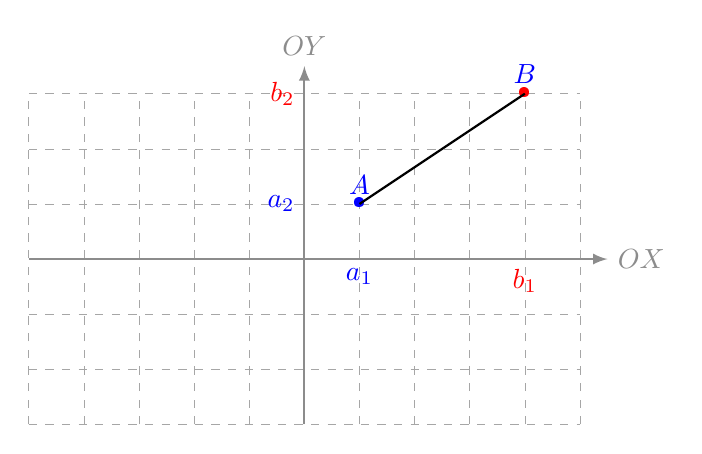
\begin{tikzpicture}[scale=0.7]
	\tikzset{>=latex}
	\draw[help lines, color=gray!70, dashed] (-5,-3) grid (5,3);
	\draw[->,thick,color=gray!90] (-5,0)--(5.5,0) node[right]{$OX$};
	\draw[->,thick,color=gray!90] (0,-3)--(0,3.5) node[above]{$OY$};

	\pgfmathsetmacro{\ax}{1}
    \pgfmathsetmacro{\ay}{1}
	\pgfmathsetmacro{\bx}{4}
    \pgfmathsetmacro{\by}{3}
	\coordinate (A) at (\ax,\ay);
	\coordinate (B) at (\bx,\by);

	\node[blue] at (A) {\textbullet};
	\node[blue,above] at (A) {\(A\)};
	\node[blue,below] at (\ax,0) {$a_1$};
	\node[blue,left] at (0,\ay) {$a_2$};

	
    \node[red] at (B) {\textbullet};
	\node[blue,above] at (B) {\(B\)};
	\node[red,below] at (\bx,0) {$b_1$};
	\node[red,left] at (0,\by) {$b_2$};
  	\draw[thick] (A)--(B) ;
	
	\end{tikzpicture}
\end{figure}
\end{frame}
%%%%%%%%%%%%%%%%%%%%%%%%%%%%%%%%%%%%%%%%%%%%%%%%%%%%
\begin{frame}[label=circulo]{}

\begin{exe}
\begin{enumerate}
\item Calcule a distância entre os pontos
\begin{enumerate}[a]
\item \(A=(2,3)\) e a origem dos sistema.
\item  \(A=(1,3)\) e \(B=(2,4)\).
\item  \(A=(1,3)\) e \(B=(-1,2)\).
\end{enumerate}
\item Determine a equação dos pontos do plano equidistantes de \(P=(1,-2)\) e \(Q=(3,4)\), em seguida faça um esboço.
 \end{enumerate}
\end{exe}
\end{frame}
%%%%%%%%%%%%%%%%%%%%%%%%%%%%%%%%%%%%%%%%%%%%%%%%%%
\begin{frame}[label=circulo]
\begin{casa}
\begin{enumerate}
\item Calcule a distância entre os ponto \(A=(2,-3)\) e \(B=(5,-1)\).
\item Determine a equação dos pontos do plano que equidistam dos pontos (1,3) e (5,1).
\end{enumerate}
\end{casa}

\end{frame}
%%%%%%%%%%%%%%%%%%%%%%%%%%%%%%%%%%%%%%%%%%%%%%%%%%%%
\begin{frame}[label=circulo]{Equação do Círculo no plano}
As coordenadas de um ponto {\color{red} \(P=(x,y)\)} de um círculo de centro  no ponto  {\color{blue}\(A=(x_0,y_0)\)} e raio \(r\) satisfazem
\[
({\color{red}x}-{\color{blue}x_0})^2+ ({\color{red}y}-{\color{blue}y_0})^2 =r^2
\]
		\begin{figure}[h]
	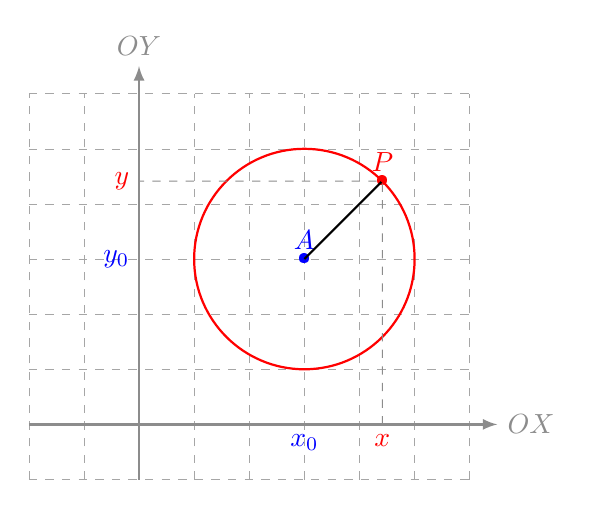
\begin{tikzpicture}[scale=0.7]
	\tikzset{>=latex}
	\draw[help lines, color=gray!70, dashed] (-2,-1) grid (6,6);
	\draw[->,thick,color=gray!90] (-2,0)--(6.5,0) node[right]{$OX$};
	\draw[->,thick,color=gray!90] (0,-1)--(0,6.5) node[above]{$OY$};

	\pgfmathsetmacro{\ax}{3}
    \pgfmathsetmacro{\ay}{3}
	\pgfmathsetmacro{\bx}{\ax + 2*cos(45)}
    \pgfmathsetmacro{\by}{\ay + 2*sin(45)}
	\coordinate (A) at (\ax,\ay);
	\coordinate (B) at (\bx,\by);

	\node[blue] at (A) {\textbullet};
	\node[blue,above] at (A) {\(A\)};
	\node[blue,below] at (\ax,0) {$x_0$};
	\node[blue,left] at (0,\ay) {$y_0$};

	
    \node[red] at (B) {\textbullet};
	\node[red,above] at (B) {\(P\)};
	\node[red,below] at (\bx,0) {$x$};
	\node[red,left] at (0,\by) {$y$};
  	\draw[thick] (A)--(B) ;

	\draw[thick, red] (A) circle (2cm) ;
	\draw[color=gray!90,dashed] (\bx,0)--(B) -- (0,\by);
	
	\end{tikzpicture}
\end{figure}
\end{frame}
%%%%%%%%%%%%%%%%%%%%%%%%%%%%%%%%%%%%%%%%%%%%%%%%%%%%
\begin{frame}[label=circulo,fragile]
\begin{pycode}
import sympy as sp
x,y=sp.symbols('x y',real=True)
x0=sp.Rational(1,2)
r=2
exp=sp.expand((x-x0)**2+y**2-r**2)
eq=sp.Eq(exp,0)
\end{pycode}
\begin{exe}
\begin{enumerate}
\item Determine a equação do círculo de centro na origem e raio 2.
\item Encontre o ponto de interseção do círculo de centro \((0,1)\) e raio 1 com a reta que que corta os eixos coordenados em \(x=1\) e \(y=2\). 
\item  Determine o centro e o raio da circunferência 
\[\pyl{eq}\]
e faça um esboço.
\end{enumerate}
\end{exe}
\end{frame}
%%%%%%%%%%%%%%%%%%%%%%%%%%%%%%%%%%%%%%%%%%%%%%%%%
\begin{frame}[label=circulo]
\begin{casa}
\begin{enumerate}
\item  Encontre o ponto de interseção do círculo de centro \((0,1)\) e raio 1 com a reta que que corta os eixos coordenados em \(x=1\) e \(y=4\). 
\item Estude o completamento de quadrados em
\item Complete o quadrado das expressões
\begin{enumerate}[a]
\item $x^2-4x$
	\item $-x^2+2x$
	\item $3x^2-9x$
\end{enumerate}
\item Determine o centro e o raio das circunferências e faça um esboço
\[2x^2+2y^2+4x-6y-19=0\]
\[x^2+y^2-4x+5y-2=0\]
e faça um esboço.
\end{enumerate}
\end{casa}
\end{frame}

